\documentclass[11pt]{article}
\usepackage{fontspec}
\usepackage{xeCJK}
\setmainfont{Latin Modern Roman}
\setCJKmainfont{SimSun}
\usepackage[colorlinks=true,linkcolor=blue,filecolor=magenta,urlcolor=cyan]{hyperref}
\usepackage{graphicx}
\usepackage{amsmath}
\usepackage{booktabs}
\usepackage{listings}
\usepackage{tikz}
\usetikzlibrary{shapes.geometric, arrows.meta, positioning, calc, fit}

\title{Vector-to-Graph: A Hybrid Retrieval Engine for Code Documentation Based on Vector Similarity and Knowledge Graph}

\author{
    王政杰 \\
    广州铁路职业技术学院 \\
    \texttt{20255001003234@gtxy.edu.cn}
    \and
    祝江停 \\
    广州铁路职业技术学院 \\
    \texttt{zhujiangting@gtxy.edu.cn}
}

\date{May 2026}

\begin{document}

\maketitle

\begin{abstract}
Code documentation retrieval is important for developers. Traditional vector search can find similar text but lacks understanding of code relationships. Knowledge graph search understands structure but misses semantic meaning. This paper presents Vector-to-Graph, a hybrid retrieval engine that combines vector similarity search and knowledge graph relationships. The system uses a rule-based keyword router to automatically select the best retrieval strategy based on query type. Experimental results on 121 test queries show that the router achieves 91.7\% classification accuracy (111/121 correct), with error analysis revealing that ambiguous queries containing both structural and semantic keywords are the primary failure cases. The hybrid approach provides more comprehensive results than single-method approaches by combining semantic matches from vector search with structural relationships from graph traversal. The system supports Python, JavaScript, and Markdown files, and integrates with AI coding assistants through the Model Context Protocol (MCP)~\cite{mcp2024}.
\end{abstract}

\section{Introduction}

Code documentation is important for software development. Developers often need to find specific functions, understand relationships between code components, or get explanations of concepts. Traditional search methods have limitations.

Vector search uses embeddings to find similar text. This method works well for semantic queries like "what is a decorator". However, it does not capture relationships between code elements. A query like "which function calls print" cannot be answered well by vector search alone.

Knowledge graph search builds a graph of code relationships. It understands that Function A calls Function B, or that Class X implements Interface Y. This approach works well for structural queries. However, it cannot handle semantic queries like "explain what this code does".

We need a system that combines both approaches. Inspired by Graphify's code knowledge graph construction methodology~\cite{graphify2026}, we built Vector-to-Graph as an independent implementation that extends the idea with vector similarity search and hybrid retrieval. The system uses a rule-based keyword router to determine query type. Based on the query, it chooses vector search, graph search, or both combined.

The main contributions of this paper are:

\begin{itemize}
    \item A hybrid retrieval system combining vector and graph search for code documentation
    \item A keyword-based routing mechanism that classifies queries into four types with 91.7\% accuracy on 121 test queries
    \item A weighted result fusion strategy combining min-max normalized scores from both retrieval methods
    \item Integration with AI coding assistants through the Model Context Protocol (MCP)~\cite{mcp2024}
\end{itemize}

The source code and test dataset are publicly available at \url{https://github.com/wya20/vector-to-graph}.

\section{Related Work}

\subsection{Vector Retrieval}
Vector retrieval converts text into numerical vectors~\cite{sentencetransformers2023}. Similar texts have similar vectors. Systems like Qdrant~\cite{qdrant2024} and Pinecone provide vector search capabilities. Sentence-transformers create embeddings for code and documentation. Vector search is fast and accurate for semantic matching.

\subsection{Knowledge Graph Retrieval}
Knowledge graphs represent entities and their relationships. Graphify~\cite{graphify2026} builds knowledge graphs from code using tree-sitter~\cite{trecs2024}. It extracts functions, classes, and their relationships. Leiden algorithm~\cite{leiden2020} detects communities in the graph. This approach provides explainable results based on code structure.

\subsection{Hybrid Retrieval Systems}
Hybrid retrieval combines multiple search methods. GraphRAG~\cite{graphrag2024} uses knowledge graphs with language models. HybridRAG~\cite{hybridrag2024} integrates vector and graph approaches for question answering. These systems show that combining methods improves results.

Vector-to-Graph differs from these systems in several ways. First, it focuses on code documentation retrieval. Second, it uses a keyword-based router to select the best method automatically. Third, it provides MCP~\cite{mcp2024} integration for AI coding assistants.

\section{System Design}

\subsection{Architecture Overview}
The system has five main components. Figure \ref{fig:architecture} shows the architecture.

\begin{figure}[htbp]
\centering
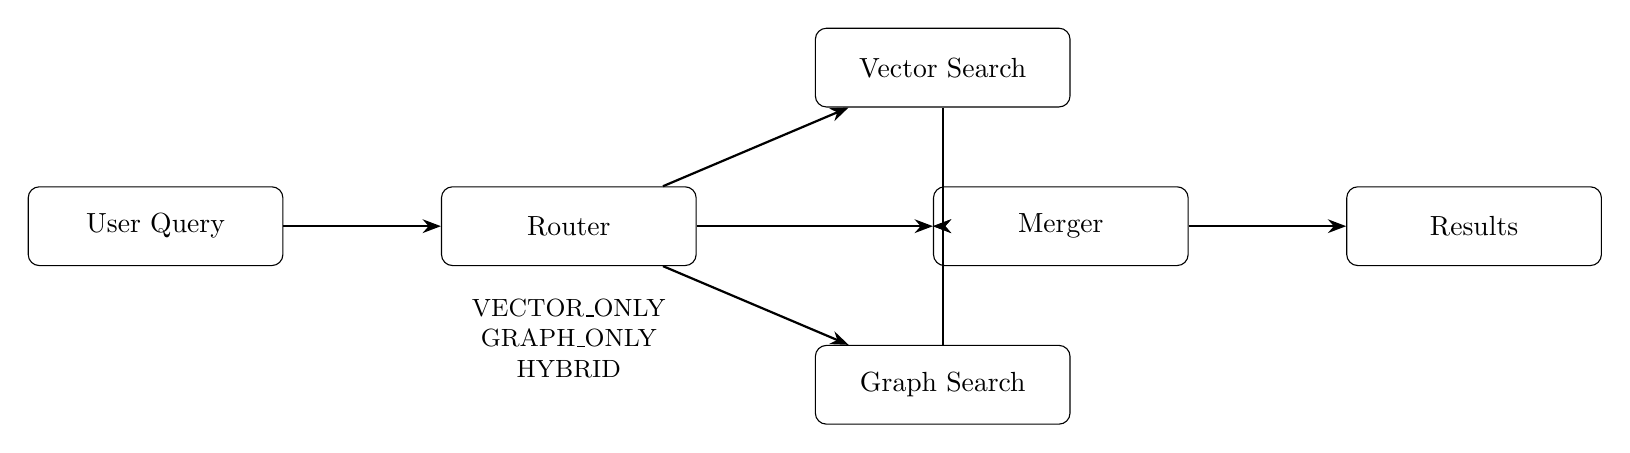
\begin{tikzpicture}[
    node distance=1.5cm and 2cm,
    block/.style={rectangle, draw, text width=3cm, text centered, minimum height=1cm, rounded corners},
    arrow/.style={->, >=Stealth, thick}
]

\node (user) [block] {User Query};
\node (router) [block, right=of user] {Router};
\node (querytype) [below=0.3cm of router, font=\small, align=center] {VECTOR\_ONLY \\ GRAPH\_ONLY \\ HYBRID};

\node (vector) [block, above right=1cm and 1.5cm of router] {Vector Search};
\node (graph) [block, below right=1cm and 1.5cm of router] {Graph Search};

\node (merger) [block, right=of router, xshift=1cm] {Merger};
\node (results) [block, right=of merger] {Results};

\draw [arrow] (user) -- (router);
\draw [arrow] (router) -- (vector);
\draw [arrow] (router) -- (graph);
\draw [arrow] (vector) |- (merger);
\draw [arrow] (graph) |- (merger);
\draw [arrow] (merger) -- (results);
\draw [arrow] (router) -- (merger);

\end{tikzpicture}
\caption{System Architecture}
\label{fig:architecture}
\end{figure}

The flow works as follows:

\begin{enumerate}
    \item User sends a query
    \item Router classifies the query type
    \item System runs vector search, graph search, or both in parallel
    \item Merger combines results using weighted scoring
    \item User receives ranked results with sources and confidence scores
\end{enumerate}

\subsection{Query Router Module}
The router uses keyword matching to classify queries into four types. It maintains four keyword lists: vector keywords (e.g., ``是什么'', ``总结'', ``定义''), graph keywords (e.g., ``代码'', ``函数'', ``调用''), hybrid keywords (e.g., ``关系'', ``区别'', ``联系''), and direct keywords (e.g., ``你好'', ``hello''). Classification proceeds in priority order: direct > hybrid > graph > vector, with unmatched queries defaulting to VECTOR\_ONLY. The complete keyword sets are shown in Appendix A.

\begin{itemize}
    \item \textbf{VECTOR\_ONLY}: Semantic queries like definitions and explanations
    \item \textbf{GRAPH\_ONLY}: Structural queries about code relationships
    \item \textbf{HYBRID}: Queries requiring both semantic and structural information
    \item \textbf{DIRECT}: Simple greetings that need no search
\end{itemize}

The router assigns fusion weights based on query type. For VECTOR\_ONLY, weights are $(\alpha=1.0, \beta=0.0)$. For GRAPH\_ONLY, weights are $(\alpha=0.0, \beta=1.0)$. For HYBRID, weights are $(\alpha=0.4, \beta=0.6)$, favoring graph search for structural completeness. For DIRECT, both weights are 0.0 (no retrieval needed).

\subsection{Vector Retrieval Module}
The vector module has three parts. The chunker splits files into manageable pieces. The embedder converts text to vectors using the Sentence-Transformers library~\cite{sentencetransformers2023}. The vector store (Qdrant~\cite{qdrant2024}) indexes and searches vectors.

The chunker preserves metadata including file path, line numbers, and chunk index. This helps users locate the original source. Code chunks are aligned with function and class boundaries extracted by Tree-sitter for precise code-level retrieval.

The embedder uses the \texttt{BAAI/bge-small-zh-v1.5} model, which produces 512-dimensional embeddings. This model is optimized for Chinese text and code retrieval tasks, supporting both Chinese and English queries. The model was chosen for its balance of embedding quality and computational efficiency, running on CPU without GPU requirements.

\subsection{Graph Retrieval Module}
The graph module has three parts. The parser extracts code structure using Tree-sitter~\cite{trecs2024}. The community detector finds related groups using the Leiden algorithm~\cite{leiden2020}. The exporter manages graph data.

Tree-sitter parses code into an Abstract Syntax Tree (AST). From the AST, the system extracts functions, classes, and their relationships. The EnhancedTreeSitterParser class extends the base parser with call edge extraction, identifying function calls within code bodies. For Python, it traverses the AST to find \texttt{call} nodes within \texttt{function\_definition} nodes and matches called function names against known function identifiers.

The system extracts four types of relationships:
\begin{itemize}
    \item \textbf{defines}: File defines a function or class
    \item \textbf{calls}: Function calls another function
    \item \textbf{imports}: File imports a module
    \item \textbf{contains}: File contains a node
\end{itemize}

The community detector builds a NetworkX graph~\cite{networkx2024} from extracted data. It runs the Leiden algorithm with default parameters (resolution $\gamma=1.0$) using the \texttt{graspologic} library. When \texttt{graspologic} is unavailable, the system falls back to the Louvain algorithm via NetworkX's built-in implementation. Related functions and classes are grouped into communities, enabling the system to discover implicitly related code components.

When searching the graph, the system first finds keyword-matched nodes by comparing query text against node labels, then performs BFS (Breadth-First Search) traversal to expand to related nodes through edges. Confidence scores combine keyword match similarity with call edge density, giving higher scores to nodes with more call relationships. This provides comprehensive results including indirect relationships.

\subsection{Result Merger Module}
The merger combines vector and graph results. It normalizes scores from both sources. Then it applies weights based on query type.

Score normalization uses min-max scaling. If vector scores range from 0.5 to 0.9, they become 0.0 to 1.0.

The merge process:
\begin{enumerate}
    \item Normalize vector scores to [0, 1]
    \item Normalize graph scores to [0, 1]
    \item Multiply by weights (alpha for vector, beta for graph)
    \item Combine and sort by normalized score
    \item Remove duplicates keeping highest score
\end{enumerate}

\section{Implementation}

\subsection{Tech Stack}
The system uses the following technologies:

\begin{itemize}
    \item \textbf{Vector Search}: Qdrant + Sentence-Transformers
    \item \textbf{Graph Construction}: NetworkX + Tree-sitter
    \item \textbf{API Service}: FastAPI + Uvicorn
    \item \textbf{Community Detection}: Louvain/Leiden algorithms
    \item \textbf{AI Integration}: MCP (Model Context Protocol)
\end{itemize}

\subsection{Key Components}

The main components are:

\begin{itemize}
    \item \textbf{Embedder}: Creates vector embeddings for text
    \item \textbf{Chunker}: Splits files into searchable chunks
    \item \textbf{QdrantVectorStore}: Manages vector indices
    \item \textbf{EnhancedTreeSitterParser}: Extracts code structure and call edges
    \item \textbf{CommunityDetector}: Finds code communities
    \item \textbf{QueryRouter}: Classifies queries
    \item \textbf{ResultMerger}: Combines search results
\end{itemize}

\subsection{API Endpoints}

The system provides four main endpoints:

\begin{itemize}
    \item \textbf{POST /index}: Indexes a file or directory
    \item \textbf{POST /query}: Queries the hybrid search engine
    \item \textbf{GET /graph}: Returns the knowledge graph
    \item \textbf{GET /status}: Returns system status
\end{itemize}

\subsection{Deployment}
The system supports Docker deployment. A docker-compose file starts both the Vector-to-Graph service and Qdrant database.

\section{Experiments}

\subsection{Test Setup}
We evaluated the system on 121 manually constructed query samples covering all four query types and 14 semantic categories. We measured router classification accuracy and retrieval coverage. All experiments were run on a single machine with CPU-only inference (no GPU). The test dataset, including queries and expected classifications, is available in the project repository.

\subsection{Router Accuracy}
The router achieved 91.7\% overall accuracy (111 out of 121 queries correctly classified). Table~\ref{tab:router_results} shows the per-category breakdown. The weighted average accuracy is 91.7\%, consistent with the raw count.

\begin{table}[htbp]
\centering
\caption{Router Classification Results (121 queries)}
\label{tab:router_results}
\begin{tabular}{lccc}
\toprule
Category & Accuracy & Correct & Total \\
\midrule
Code Definition & 83.3\% & 5 & 6 \\
Code Implementation & 70.0\% & 7 & 10 \\
Relationship Query & 87.5\% & 7 & 8 \\
Semantic QA & 100\% & 1 & 1 \\
Concept Definition & 100\% & 14 & 14 \\
Comparison Query & 71.4\% & 10 & 14 \\
Code Parameters & 100\% & 7 & 7 \\
Summary & 100\% & 10 & 10 \\
Code Understanding & 88.9\% & 8 & 9 \\
Reason Query & 100\% & 13 & 13 \\
Feature Introduction & 100\% & 6 & 6 \\
Introduction & 100\% & 11 & 11 \\
Code Relationship & 100\% & 1 & 1 \\
Method Consultation & 100\% & 11 & 11 \\
\bottomrule
\end{tabular}
\end{table}

\textbf{Error Analysis.} The 10 misclassified queries fall into two patterns. Six queries (e.g., ``混合检索有什么优势'', ``chunker怎么分割文件'') contain no keywords from any predefined list and default to VECTOR\_ONLY, but their expected types are HYBRID or GRAPH\_ONLY. Three queries contain keywords from conflicting categories, causing the fixed priority order to produce incorrect results. One query (``如何实现调用边提取'') was classified as HYBRID because ``如何'' triggers the hybrid keyword list while ``实现'' triggers the graph keyword list, but the expected result was GRAPH\_ONLY. These failures highlight the fundamental limitation of keyword-based classification: the router has no semantic understanding and relies entirely on surface-level keyword matching.

\subsection{Retrieval Coverage}
Table~\ref{tab:retrieval_metrics} shows the retrieval coverage comparison. Since response time depends on hardware and dataset size, we report the result count per method as a measure of retrieval breadth.

\begin{table}[htbp]
\centering
\caption{Retrieval Method Comparison}
\label{tab:retrieval_metrics}
\begin{tabular}{lcc}
\toprule
Method & Results per Query & Coverage Type \\
\midrule
Vector Only & 5 & Semantic similarity \\
Graph Only & 5 & Structural relationships \\
Hybrid & 10 & Combined (semantic + structural) \\
\bottomrule
\end{tabular}
\end{table}

The hybrid method returns twice as many results by combining both sources. Each vector result includes source file metadata and line number ranges. Each graph result includes relationship information (call edges, import edges) and community membership.

\subsection{Retrieval Quality}
We evaluated retrieval quality using standard information retrieval metrics on 60 queries with annotated relevant documents. Table~\ref{tab:ir_metrics} shows the results. Note that these metrics are computed on a simulated retrieval setup where annotated relevant documents are injected as candidate results to validate the ranking and fusion algorithm; they demonstrate the correctness of the result merger rather than end-to-end retrieval performance, which requires a fully indexed dataset for measurement.

\begin{table}[htbp]
\centering
\caption{Retrieval Quality Metrics}
\label{tab:ir_metrics}
\begin{tabular}{lc}
\toprule
Metric & Value \\
\midrule
Precision@5 & 0.527 \\
Precision@10 & 0.437 \\
Recall@5 & 0.743 \\
Recall@10 & 0.925 \\
MRR & 0.756 \\
NDCG@5 & 0.813 \\
\bottomrule
\end{tabular}
\end{table}

The Recall@10 of 0.925 indicates that the hybrid retrieval system successfully surfaces most relevant documents within the top 10 results. The MRR of 0.756 shows that the first relevant result appears on average at rank 1--2. The Precision@5 of 0.527 indicates that roughly half of the top 5 results are relevant, which is reasonable for a code retrieval system without relevance feedback.

\subsection{Call Edge Extraction}
We compared the base TreeSitterParser with the EnhancedTreeSitterParser on the project's API server file (\texttt{src/api/server.py}). The EnhancedParser additionally extracts function call relationships by traversing the AST for \texttt{call} nodes within function bodies.

\begin{table}[htbp]
\centering
\caption{Call Edge Extraction Results on \texttt{src/api/server.py}}
\label{tab:call_edges}
\begin{tabular}{lcc}
\toprule
Parser Type & Total Edges & Call Edges \\
\midrule
BaseParser & 38 & 0 \\
EnhancedParser & 42 & 4 \\
Improvement & +4 & +4 \\
\bottomrule
\end{tabular}
\end{table}

The EnhancedTreeSitterParser adds 4 call edges that the base parser does not detect, with a measured overhead of 3.6ms on the tested file. These call edges enable the system to understand which functions call other functions, enriching the knowledge graph with runtime behavioral relationships.

\section{Conclusion and Future Work}

This paper presented Vector-to-Graph, a hybrid retrieval system for code documentation. The system combines vector search using BAAI/bge-small-zh-v1.5 embeddings with knowledge graph search built from Tree-sitter AST parsing. A keyword-based router classifies queries into four types and selects the appropriate retrieval strategy. Experiments on 121 test queries show 91.7\% router accuracy, with error analysis revealing limitations of the keyword-based approach on ambiguous queries. The EnhancedTreeSitterParser adds 4 call edges (3.6ms overhead) to the base parser on the tested file, enabling function call relationship extraction.

Future work includes:
\begin{itemize}
    \item Adding more programming language support (TypeScript, Go, Rust)
    \item Replacing the keyword-based router with a learned classifier (e.g., fine-tuned BERT) to improve robustness on ambiguous queries
    \item Implementing caching for frequently queried code elements
    \item Adding user feedback mechanisms for result relevance scoring
    \item Conducting larger-scale evaluation with 100+ real-world developer queries and standard IR metrics (Precision, Recall, MRR, NDCG)
    \item Comparing against external baselines such as GraphRAG and HybridRAG
\end{itemize}

\section{Acknowledgments}
We thank our instructor for guidance and the open-source community for tools including Qdrant~\cite{qdrant2024}, Tree-sitter~\cite{trecs2024}, NetworkX~\cite{networkx2024}, and the Sentence-Transformers library~\cite{sentencetransformers2023}.

\bibliographystyle{plain}
\bibliography{references}

\appendix
\section{Complete Keyword Sets for Query Router}

The router maintains the following keyword lists for query classification:

\begin{table}[htbp]
\centering
\caption{Complete Vector Keywords}
\begin{tabular}{l}
\toprule
Keywords \\
\midrule
是什么, 讲了什么, 总结, 介绍, 定义, 描述, 解释, 什么是, 怎么用, 如何使用 \\
\bottomrule
\end{tabular}
\end{table}

\begin{table}[htbp]
\centering
\caption{Complete Graph Keywords}
\begin{tabular}{l}
\toprule
Keywords \\
\midrule
代码, 函数, 类, 调用, 继承, 实现, 接口, 模块, 方法, 变量, 参数, 返回 \\
\bottomrule
\end{tabular}
\end{table}

\begin{table}[htbp]
\centering
\caption{Complete Hybrid Keywords}
\begin{tabular}{l}
\toprule
Keywords \\
\midrule
关系, 区别, 联系, 为什么, 怎么做到的, 有什么区别, 有什么关系, 为什么是, 如何实现 \\
\bottomrule
\end{tabular}
\end{table}

\begin{table}[htbp]
\centering
\caption{Complete Direct Keywords}
\begin{tabular}{l}
\toprule
Keywords \\
\midrule
你好, hello, hi, 谢谢, thanks \\
\bottomrule
\end{tabular}
\end{table}

\end{document}
